%
% waveequation.tex -- the wave equation
%
% (c) 2019 Prof Dr Andreas Mueller
%
\rhead{Wave equation}
\section{Wave equation\label{beispiele:wellengleichung}}
\index{wave equation}
In the simplest form, this equation describes the motion
of a string of a guitar or a piano, or the air column of a 
wind instrument.
It can be generalized to vibration of a membrane or the fluid inside
an arbitrary threedimensional volume.
Electromagnetic waves can be modelled with this equation just as
well as the waves on the surface of a lake.

\subsection{The differential equation of a vibrating string}
\index{string}
Let a thin string with linear mass density $\mu$ be mounted between
the points $x=0$ and $x=l$.
The force $F$ at the end points of the string maintains its tension.
We ask for a partial differential that describes the motion of a
string after we bring it into a certain shape and let it go at time $t=0$

The state of the string at any time can be described by a function
$u(x,t)$, which measures the deflection of the string from the straight
line between the two end points.
We need to find a differential equation for the function $u$.

From this problem description we can already derive some information
about the solution.
We note that the end points of the string are fixed, so
\[
u(0,t)=u(l,t)=0\quad\forall t\ge 0.
\]
We call this a boundary condition.
At time $t=0$ the string is supposed to have a given shape.
This is the situation of the guitar player who plucks a string and then
lets it go.
Mathematically we can formulate this as the initial condition
\[
u(x,t) = f(x)\qquad 0 < x < l.
\]
A piano however works differently, at $t=0$ it imparts a certain velocity
profile on the string, or in mathematical form
\[
\frac{partial}{\partial t}u(0,x) = g(x),\qquad 0<x<l.
\]

\begin{figure}
\begin{center}
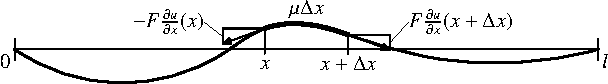
\includegraphics[width=\hsize]{../common/images/saite-1}
\end{center}
\caption{Derivation of the differential equation of a vibrating string
\label{saite}}
\end{figure}
To derive the equation of motion of a vibrating string, we consider
a small section of the string between coordinates $x$ and $x+\Delta x$
(figure \ref{saite}).
Newton's law says that the acceleration of this piece of string 
is proportional to forces acting on it, with the mass as proportionality
factor.
The mass of this piece of the string is $m=\mu\Delta x$.
At each end of the segment, a force of absolute value $F$ pulls the piece
outward, but these forces don't necessarily have the same direction,
resulting in a vertical force component.
This component turns out to be
\[
F\frac{\partial u}{\partial x}(x+\Delta x)-F\frac{\partial u}{\partial x}(x).
\]
Since the acceleration of the string segment is
$\frac{\partial^2u}{\partial t^2}$
we obtain the equation of motion
\begin{align*}
\mu\Delta x\frac{\partial^2u}{\partial t^2}(x)&=
F\frac{\partial u}{\partial x}(x+\Delta x)-F\frac{\partial u}{\partial x}(x)\\
\Rightarrow\qquad
\frac{\mu}{F}\frac{\partial^2u}{\partial t^2}(x)&=
\frac1{\Delta x}\left(\frac{\partial u}{\partial x}(x+\Delta x)-\frac{\partial u}{\partial x}(x)\right)
\end{align*}
By going to the limit 
$\Delta x\to 0$ we obtain the partial differential equation
\[
\frac{\partial^2u}{\partial t^2}=\frac{F}{\mu}\frac{\partial^2u}{\partial x^2}.
\]
The coefficient
$\frac{F}{\mu}$
has the dimension of a velocity squared, it is the velocity by which waves
propagate along the string.

\subsection{The differential equation of an organ pipe}
The analysis of the vibrating string carries over almost unchanged
to a pipe organ (or any other wind instrument).
The deflection of the string is replaced by a deviation of the pressure.
We then obtain the wave equation
\[
\frac{\partial^2p}{\partial t^2}=
a^2\frac{\partial^2p}{\partial x^2}
\]
Again, $a$ is the speed of sound.

The boundary conditions, however, turn out to be more complicated and more
interesting.
If the end of the pipe is closed, then the air cannot move at this end.
Because movement of the air in the pipe is always associated with pressure
differences, we conclude that there cannot be a pressure gradient at the
end of the pipe in this case.
This leads to the so called Neumann boundary condition
\[
\frac{\partial}{\partial x}p(x_0,t) = 0\qquad t>0.
\]
If the pipe is open, then there is nothing that keeps the air in the pipe,
air can move freely, and the pressure is always as the surrounding air.
This leads to the so called Dirichlet boundary condition
\[
u(x_0,t)=0\qquad t>0.
\]

\subsection{Wave equation in two and three dimensions}
In analogy with the differential equation of a string we can derive the
equation of motion of a membrane fixed around its perimeter.
Let $G$ be a domain in $\mathbb R^2$, and let $\gamma\subset G$ be
the boundary curve of the domain, i.~e.~$\gamma = \partial G$.
Then the deviation of the membrane from zero position is a function
\[
 u \colon G\times \mathbb R_{t \ge 0}\to\mathbb R\colon (x,y,t)\mapsto  u (x,y,t)
\]
The membrane is fixed at the boundary, so $u$ has to satisfy the
boundary conditions
\[
 u (x,y,t)=0\qquad \forall (x,y)\in\gamma,\quad t\ge 0.
\]
The function satisfies the differential equation
\[
\frac{\partial^2 u }{\partial t^2}
=
c^2\left(\frac{\partial^2 u }{\partial x^2}
+
\frac{\partial^2 u }{\partial y^2}\right).
\]
The solution is only determined, if we know the initial shape of the
membrane and its velocity. 
This leads to the initial conditions
\[
 u (x,y,0)=f(x,y)\qquad \forall (x,y)\in G.
\]

In three dimensions, the wave equation becomes
\[
\frac{\partial^2 u }{\partial t^2}
=c^2\left(\frac{\partial^2 u }{\partial x^2}
+\frac{\partial^2 u }{\partial y^2}
+\frac{\partial^2 u }{\partial z^2}
\right).
\]
The additional data required also becomes a bit more involved.
First we have to define a domain 
$G\subset \mathbb R^3$ in threedimensional space.
The boundary of this volume must be a sufficiently smooth surface.
The solution then has to satisfy the boundary conditions
$u(x,y,z,t) = 0$ for points
$(x,y,z)\in \partial G$ on the boundary surface of $G$.

\subsection{The Laplace operator\label{beispiele:laplaceoperator}}
In all the problems discussed so far, the Laplace operator,
also called laplacian,
\[
\Delta
=
\begin{cases}
\displaystyle
\frac{\partial^2}{\partial x^2}
+\frac{\partial^2}{\partial y^2}&\qquad\text{2 Dimensionen}\\
\\
\displaystyle
\frac{\partial^2}{\partial x^2}
+\frac{\partial^2}{\partial y^2}
+\frac{\partial^2}{\partial z^2}&\qquad\text{3 Dimensionen}
\end{cases}
\]
appeared.
In fact, up to a constant factor, this is the only linear operator involving
only second derivatives that is invariant with arbitrary rotations of the
coordinate system.
This means that this is the only operator that can have a physical
meaning independent of the choice of coordinate system.

